\documentclass[a4paper,titlepage]{article}

%\setcounter{secnumdepth}{5}

% Swedish support
\usepackage[utf8]{inputenc}
\usepackage[T1]{fontenc}
\usepackage[english,swedish]{babel}

% Useful utilities
\usepackage{amsmath}
\usepackage{amsfonts}
\usepackage{amsthm}
\usepackage{amssymb}
\usepackage{graphicx}
\usepackage{microtype}
\usepackage{hyperref}
\usepackage[swedish]{cleveref}
\usepackage{siunitx}
\usepackage{tikz}
\usepackage{color}
\usepackage{pgfplots}
\usepackage{mathtools}
%\usepackage{natbib}
\usepackage{algorithm} 
\usepackage{algpseudocode}

%\bibpunct{[}{]}{,}{n}{}{;}

\pgfplotsset{compat=1.10}

%====================  defined macros  ======================================
\setlength\extrarowheight{2pt}

\algnewcommand{\LineComment}[1]{\State \(\triangleright\) #1}

\providecommand{\ceil}[1]{\left \lceil #1 \right \rceil }
\providecommand{\floor}[1]{\left \lfloor #1 \right \rfloor }

% \newcommand{\C}[1]{\Vert #1 \Vert}
\newcommand{\N}{\mathbb{N}}
\newcommand{\C}[1]{\mathfrak C \left( #1 \right)}
\newcommand{\FIX}[1]{{\color{red} \bf #1}}
\renewcommand{\O}{\mathcal {O}}
\def\lc{\left\lceil}   
\def\rc{\right\rceil}
\def\lf{\left\lfloor}   
\def\rf{\right\rfloor}

%====================  style theorems  ======================================

\newtheorem{theorem}{Sats}
\newtheorem{lemma}{Lemma}
\newtheorem{conjecture}{Förmodan}
\newtheorem{proposition}{Proposition}
\newtheorem{corollary}{Korollarium}
\theoremstyle{definition}
\newtheorem{definition}{Definition}
\newtheorem{statement}{Påstående}
\newtheorem{problem}{Problem}
\newtheorem{fact}{Faktum}
\newtheorem*{hypot}{Hypotes}

\newcommand*\foobar{
\includegraphics[height=2pt]{babyseal}}
%\catcode`\,=13 % make "." active
%\def,{\foobar}
\renewcommand\cdot{\mathbin{\raisebox{2pt}{\foobar}}}
%====================  Document starts here  ======================================

\title{En studie av heltalens komplexitet}
\author{Lisa Vällfors \and Adrian Becedas \and Joakim Blikstad}

\begin{document}

\maketitle
\selectlanguage{english}
\begin{abstract}
    In this report we will study the complexity of the natural numbers. 
    The first part of the report discusses and presents proofs and illustrations for the bounds of functions
    concerning integer complexity.
    The report also investigates specific groups of integers, such as prime numbers and
    powers of 3, presenting narrower bounds and explicit formulas.
    Finally the report explains several algorithms, of varying intricacy and efficiency, for finding integer
    complexity.
    
\end{abstract}
\selectlanguage{swedish}

\tableofcontents 
\newpage

\section{Inledning}
    
    \FIX{BRÖDTEXT!!!!}

    \begin{definition}
       Vi definierar komplexiteten av ett positivt heltal $n$ som det minimala
       antalet $1$:or som krävs för att skriva $n$ med hjälp av addition,
       subtraktion och parenteser. Vi låter $\C{n}$ beteckna komplexiteten av
       $n$. 
    \end{definition}
    \begin{center}
 \begin{tabular}{| l | l | l | }
    \hline
    n & $\C{n}$ & Exempel på minimal representation  \\ \hline
    1 & 1 & 1  \\ \hline
    2 & 2 & 1+1  \\ \hline
    3 & 3 & 1+1+1  \\ \hline
    4 & 4 & 1+1+1+1  \\ \hline
    5 & 5 & (1+1)(1+1)+1  \\ \hline
    6 & 5 & (1+1)(1+1+1)  \\ \hline
    7 & 6 & (1+1)(1+1+1)+1  \\ \hline
    8 & 6 & (1+1)(1+1)(1+1)  \\ \hline
    9 & 6 & (1+1+1)(1+1+1)  \\ \hline
    10 & 7 & (1+1+1)(1+1+1)+1  \\ \hline
    11 & 8 & (1+1+1)(1+1+1)+1+1  \\ \hline
    12 & 7 & (1+1)(1+1)(1+1+1)  \\
    \hline
    \end{tabular}
\end{center}
    Notera att den minimala representationen inte nödvändigtvis är unik.
    Exempelvis kan 4 även skrivas som $(1+1)(1+1)$. Vi kan direkt inse att $\C{n} \le n$
    eftersom man alltid kan använda den triviala representationen med endast addition.

	  \subsection{Motivation}
	
	Frågor om storleken på heltalens komplexitet har ofta enkla formuleringar som är enkla att 	förstå utan en matematisk utbildning.
    Svaren på frågorna verkar dock vara betydligt svårare och kan ge insikt i ett antal andra frågor.	
	
	\subsubsection{Ett exempel}


	Clay Mathematical Institute tillkännagav år 2000 en prispott på 7 miljoner amerikanska dollar 	för lösningar till 7 olösta problem, 1 miljon vardera. Ett av dessa viktiga problem är $P \stackrel{?}{=} NP$, ett av de viktigaste olösta problemen inom datalogin idag.

		
	$P$ och $NP$ kan illustreras med följande exempel. 
	Givet är ett alfabet A,
	en mängd A* av alla finita ord som kan skrivas med A,
	ett språk S som är en delmängd av A*. Då
	tillhör S P omm det existerar en algoritm T och ett polynom F så att T ger T(x)=1 om x är ett element ur S och T(x)=0 om x ej är ett element ur S,
    samt att T ger T(x) på en tid 	$\le$ F(|x|), där |x| betecknar längden av ordet x.
	S tillhör NP omm det existerar en algoritm T och ett polynom F så att det för alla x existerar ett
    y så att |y|$\le$F(|x|) och T ger T(x,y)=1 om x år ett element ur S på en tid $\le$ F(|x|) och T
	ger T(x,y)=0 omm x ej tillhör S. Problemet $P \stackrel{?}{=} NP$ frågar då om alla instanser i NP också är i P.
    
    Tidskomplexiteten för att räkna ut komplexiteten av ett 
	givet heltal är kopplat till problemet $P \stackrel{?}{=} NP$.
    
	\FIX{SE ÖVER DETTA!} \\
	En koppling är att $P = NP$  implicerar att det existerar en algoritm T för att räkna ut komplexiteten av heltal n som har tidskomplexitet $\le$  $C (\log n)^k$. 
	En annan koppling är att $P = NP$  implicerar att det inte existerar en talföljd av naturliga tal 
	$a_i$ så att $\underset{i\to\infty}{\lim} \frac{\C{a_i}}{\ln{a_i}} \le \frac{3}{\ln{3}}$
	 

    \subsection{Frågeställningar}
            Trots att definitionen av $\C{n}$ är så pass enkel finns det många
            frågor som kan ställas kring den. Frågeställningarna är av
            varierande svårighet, där vissa undersökts mycket men ännu är olösta, medan
            andra är helt outforskade.
             I denna rapport behandlas följande frågeställningar.
            \begin{itemize}
            \item Finns det övre och undre gränser och hur tajta är dessa?
            \item Hur fördelar sig $\frac{\C{n}}{\ln{n}}$?
            \item Kan man få tajtare gränser för specifika tal, alternativt få
                en explicit formel?
                \begin{itemize}
                    \item kvadrattal
                    \item primtal
                    \item 2 potenser
                    \item 3 potenser

                \end{itemize}
            \item Hur kan man bäst generera talen, vad är bästa tidskomplexitet
                man kan uppnå?
        %    \item (Kommer sekvensen ändras om man tillåter fler operationer
        %        utöver addition och multiplication?)
        %        \begin{itemize}
        %            \item subtraktion 
        %            \item exponensiering
        %        \end{itemize}
        \end{itemize}


\section{Analys \FIX{titel}}
    Vid undersökning av funktioner är en intressant fråga ofta om det går att finna någon övre eller undre gräns.
    Som vi ska se i senare avsnitt kan gränserna användas för att konstruera snabbare algoritmer. 
    I detta avsnitt presenteras de övre och undre gränser som redan upptäckts,
    samt bevis för dessa. Vidare undersöks gränserna genom att funktionen $ L(n) = \frac{\ln(n)}{\C{n}}$ introduceras.
    Slutligen beskrivs några hypoteser kring specifika typer av tal. 

    \subsection{Övre gräns}
    \label{ovregrans}
    Den hittills bästa övre gränsen upptäcktes av J. Arias de
    Reyna~\cite{spansk}.
    Nedan presenteras ett bevis för denna.
    \begin{definition}
        Vi definierar funktionen $A:\N\to\N$ på följande sätt:
        $$ A(n) = \left\{ \begin{matrix*}[l] 1 & \text{om } n=1 \\ 1+A(n-1) & \text{om $n$ är primtal} \\ \sum_{i=1}^kA(p_i) & \text{om } n=p_1p_2 \ldots p_k \end{matrix*} \right. $$
    \end{definition}

    Man ser att $A(n)\ge\C{n}$ då man alltid kan konstruera tal med
    funktionen~$A$. Värt att nämna är att det existerar $n$ där $A(n)\neq\C{n}$.
    Vi bevisar en övre gräns på $A(n)$ i syftet att få en övre gräns på $\C{n}$.

    \begin{lemma}
        $A(n)\le 3 \log_2{n}$ \quad för alla $n\ge2$
        \label{lemma:adrian}
    \end{lemma}
    \begin{proof}
        Vi utför stark induktion på $n$. Basfallet $n=2$ ger:
        \begin{align*}
            VL &=A(2)=1+A(1)=2\\
            HL &= 3 \log_2{2}=3 
        \end{align*}
        Alltså $VL \le HL$ som vi ville.
        Nu antar vi att \cref{lemma:adrian} gäller för alla $n \le k$. Vi vill
        visa att den även gäller för $n=k+1$.
        Vi har två fall, då $k+1$ är primtal och då det är sammansatt.

        $k+1$ är primtal ger enligt induktionsantagandet (notera $k$ är jämnt
        då $k+1$ är ett primtal $\ge3$):
        $$A(k+1) = 1 + A(k) = 1+2+A\left(\frac{k}{2}\right) \le 3 + 3 \log_2\frac{k}{2}$$
        Genom att använda identiteten \,$\log \frac{a}{b}=\log a -\log b$\, fås:
        $$ 3 + 3 \log_2\frac{k}{2} = 3 + 3\log_2 k - 3\log_2 2 = 3\log_2 k < 3\log_2 (k+1)$$
        vilket ger att $A(k+1)\le 3\log_2 (k+1)$ om $k+1$ är ett primtal.

        Om $k+1$ är sammansatt kan vi skriva $k+1 = ab$ för heltal $a,b \ge 2$.
        Vi får då enligt induktionsantagandet:
        $$A(k+1) = A(a)+A(b) \le 3(\log_2a + \log_2b) = 3\log_2 ab = 3\log_2
        (k+1)$$ Alltså gäller även $A(k+1) \le 3\log_2 (k+1)$ om $k+1$ är
        sammansatt. Enligt induktionsprincipen är alltså \cref{lemma:adrian} nu
        bevisat.
    \end{proof}

    Beviset ger alltså att $\C{n}\le A(n)\le 3\log_2 n$ för alla $n\ge2$. Denna
    gräns är dock inte särskilt bra, men ingen bättre gräns har hittats.

    \subsection{Undre gräns}
    \label{undregrans}

    Att bevisa en bra undre gräns till $\C{n}$ är något svårare.
    Idén är att man låter $E(m)$ vara det största heltalet som har komplexitet $m$.
    Detta betyder att $\C{E(m)} = m$ och att för alla $k > E(m)$ så är $\C{k}>m$.
    Med induktion kan man bevisa den slutna formeln (för $n>1$):
    $$ E(n) = \left\{ \begin{matrix*}[l] 3^k & \text{om } n=3k \\
                             4\cdot3^{k-1} & \text{om } n=3k+1 \\
                                 2\cdot3^k & \text{om } n=3k+2 \end{matrix*}
            \right.$$
    Man låter då funktionen $B$ vara följande:
    $$ B(n) = \left\{ \begin{matrix*}[l] 3k & \text{om } n\in[3^k,4\cdot3^{k-1}) \\
                                       3k+1 & \text{om } n\in[4\cdot3^{k-1},2\cdot3^k) \\
                                       3k+2 & \text{om } n\in[2\cdot3^k,3^{k+1}) \end{matrix*}
            \right.$$
    Enligt ovanstående är $B(n)\le\C{n}$.
    \begin{lemma}
        $B(n)\ge 3\log_3 n$ \quad för alla $n\ge1$
    \end{lemma}
    \begin{proof}
       Om man falluppdelar för att $n$ ligger i respektive av de tre grupperna
       får man enkelt fram att lemmat gäller genom induktion.
    \end{proof}

    Eftersom $B(n)\le\C{n}$ följer av lemmat således att $\C{n}\ge 3\log_3 n$ vilket är
    den bästa kända undre gränsen för $\C{n}$.

    \subsection{Diskussion kring gränserna}

    I ovanstående två avsnitt bevisades följande gränser på
    heltalskomplexiteten:
    $$3\log_3 n \le \C{n}\le 3\log_2 n \quad \text{($n\ge2$)}$$
    
    \begin{figure}[H]
        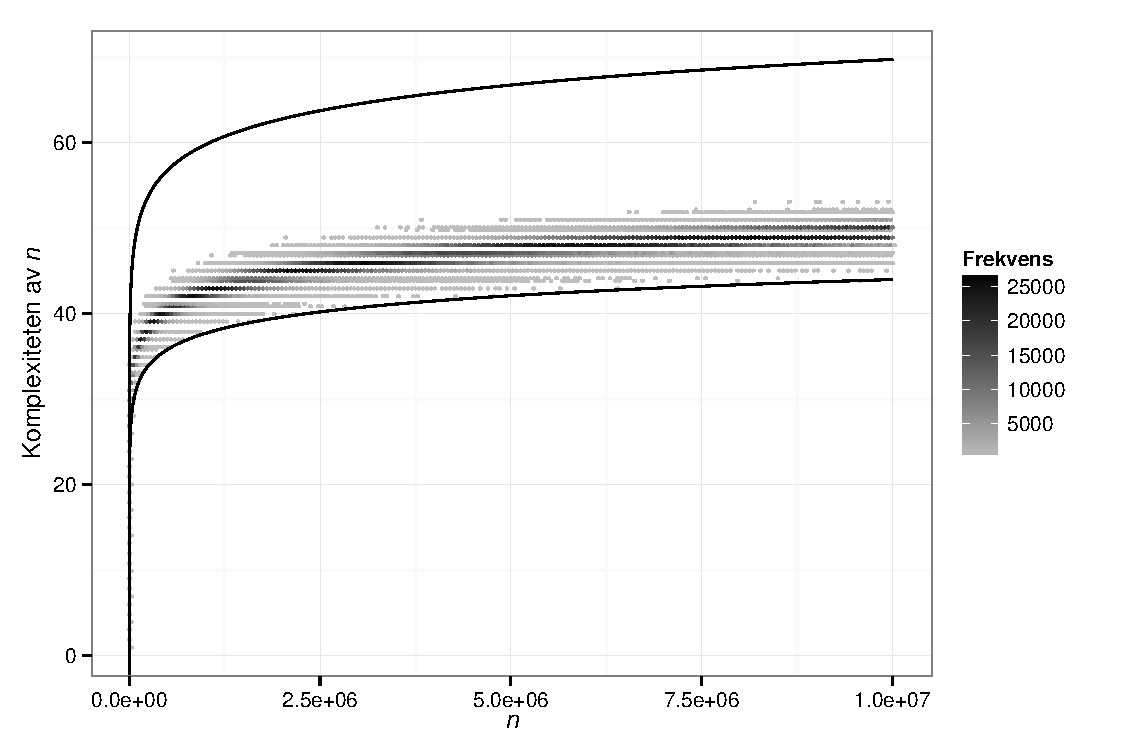
\includegraphics[width=\textwidth]{grafer/bounds}
        \caption{Graf över $\C{n}$ med den övre gränsen $3\log_2(n)$ och den undre $3\log_3(n)$}
        \label{bounds}
    \end{figure}

    Som man ser i \cref{bounds} är den undre gränsen så tight som det går, åtminstone som logaritmisk funktion. Den övre däremot ser ut att kunna
    förbättras en del, och där finns möjlighet för vidare forskning i framtiden.

    \begin{figure}[H]
        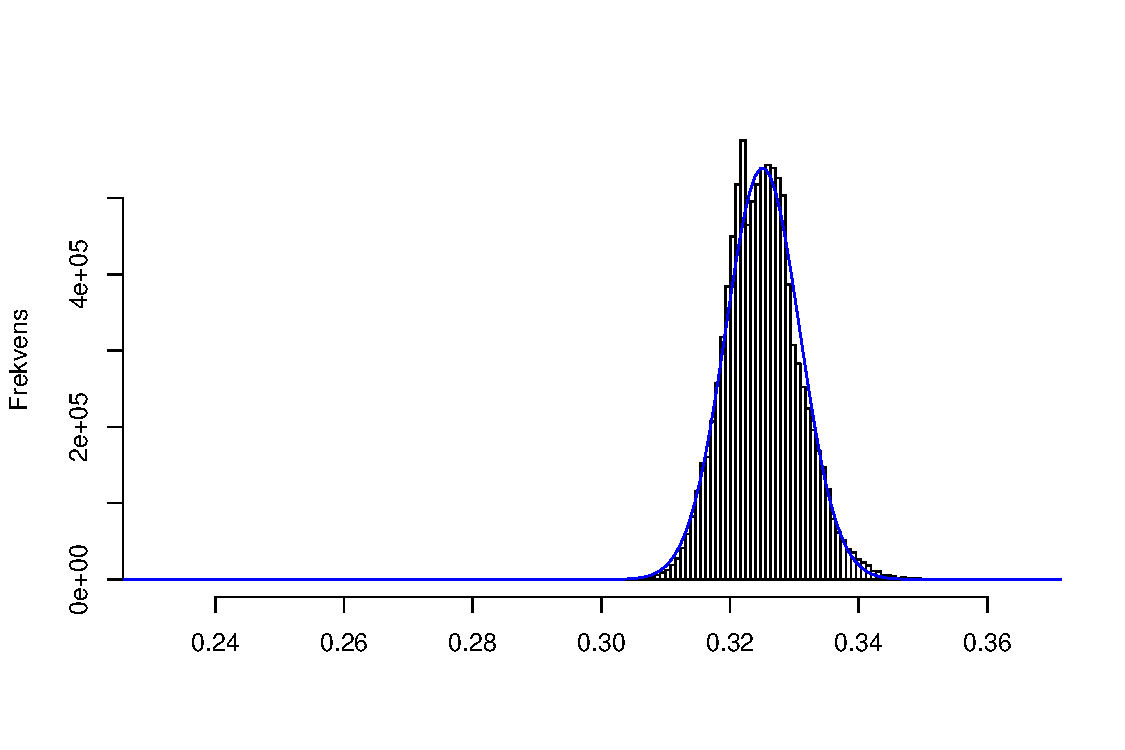
\includegraphics[width=\textwidth]{grafer/normhist}
        \caption{Histogram över $\frac{\ln(n)}{\C{n}}$ för alla $n\le10^7$ med anpassad normalfördelningskurva}
        \label{normhist}
    \end{figure}

    En annan intressant fråga är hur nära gränserna talen generellt sett ligger.
    Låt $ L(n) = \frac{\ln(n)}{\C{n}}$. Enligt \cref{undregrans} gäller

    $$3\log_3 n \le \C{n} $$
    $$\frac{\log_3 n}{\C{n}} \le \frac{1}{3}$$
    $$\frac{\ln n}{\C{n}} \le \frac{\ln 3}{3}$$
    $$ L(n) \le \frac{\ln 3}{3} \approx 0.366$$

    Den undre gränsen för $\C{n}$ ger alltså en övre gräns för värdet på $L(n)$, och desto närmre
    $\C{n}$ ligger den undre gränsen, desto närmre kommer $\L{n}$ ligga denna övre gräns.

    På samma sätt kan den övre gränsen för $\C{n}$ användas för att ge den undre gränsen

    $$ L(n) \ge \frac{\ln 2}{3} \approx 0.231 $$

    Något vi frågade oss då vi såg det histogram av $L(n)$ som ses ovan, var huruvida funktionen var normalfördelad.
    Det vore möjligt att den höga topp respektive låga dal bara var tillfälligheter som berodde på att vi plottade över för få tal.
    Som synes i \cref{normhist} går det relativt bra att anpassa en normalfördelning (den blå kurvan).
    För att undersöka huruvida histogrammets form är permanent och kommer förtydligas vid större intervall,
    eller om det kommer jämnas ut, plottades histogram över två olika intervall, se \cref{redblue}. De båda histogrammen är förvillande
    lika, men formen är något förskjuten. Faktum är att dalen i det röda histogrammet sammanfaller med högsta punkten
    i det blåa. Vad som orsakar att formen blir så här fann vi inget svar på. Formen blir inte mer och mer förskjuten till höger
    då den övre gränsen blir högre, som \cref{redblue} skulle kunna antyda. Istället varierar positionen fram och tillbaka, utan
    något uppenbart mönster.

    \FIX{ÄNDRA FÄRG PÅ REDBLUE}
    \begin{figure}[H]
        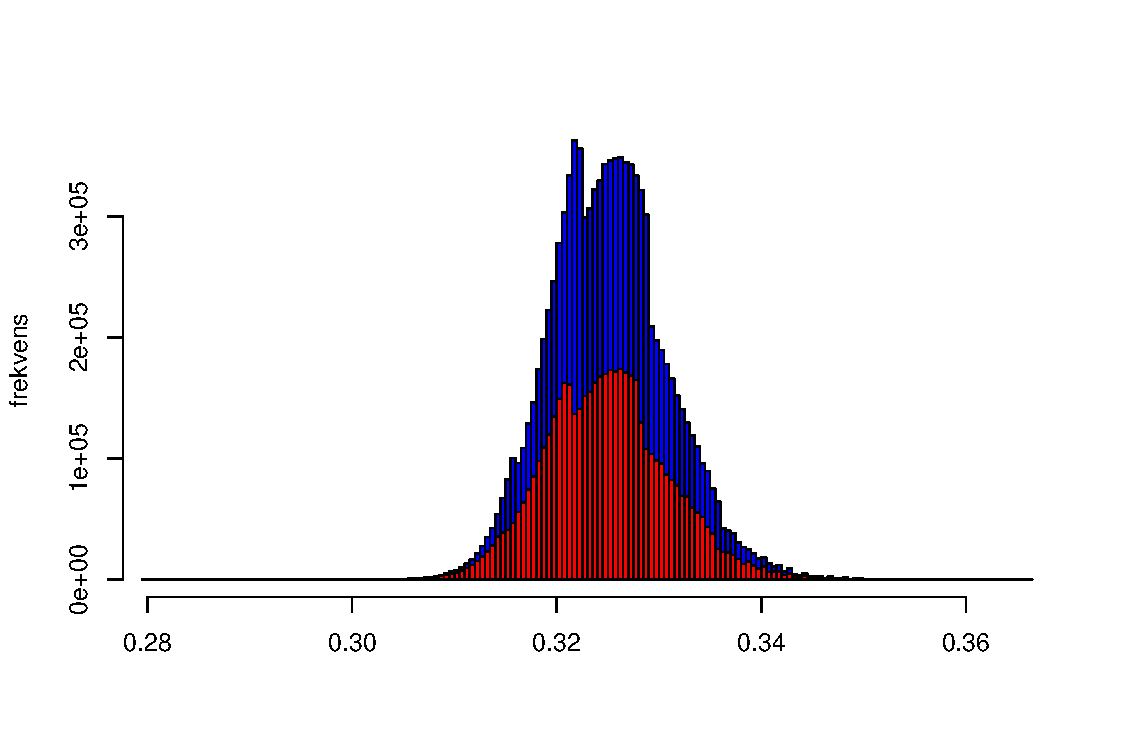
\includegraphics[width=\textwidth]{grafer/redblue}
        \caption{Histogram över $\frac{\ln(n)}{\C{n}}$. I blått $n\le10^7$ och rött $n\le5\protect\cdot10^6$}
        \label{redblue}
    \end{figure}

    \subsection{Speciella typer av tal}
    \FIX{LÄGG TILL EXEMPEL + BRÖD} \\
    Då ingen explicit formel för $\C{n}$ har hittats, finns ett intresse i att undersöka huruvida
    samband existerar för specifika typer av tal. 
        \subsubsection{Kvadrattal}
        \begin{hypot}
            $\C{n^2}=2\cdot\C{n}$ \quad för alla $n\ge1$ \\
            Denna hypotes bevisas falsk genom motexemplet $n=5^4$ vilket ger $\C{n}=20$
            och $\C{n^2}=39<40=2\cdot\C{n}$.
        \end{hypot}

        \subsubsection{Primtal}
        \begin{hypot}
            $\C{p}=\C{p-1}+1$ \quad för alla primtal $p$ \\
            Detta är något som troddes vara sant väldigt länge. Matematikern
            Richard Guy inkluderade denna frågeställning i sin bok \cite{guy}.
            Med hjälp av de betydligt snabbare algoritmerna kunde man dock finna
            det minsta motexemplet $p = \num{353942783}$ för vilket $\C{p} = 63
            < 64 = \C{p-1}+1$. \cite{ospansk}
        \end{hypot}

        \subsubsection{3-potenser}
        \begin{hypot}
            $\C{3^k}=3k$ \quad för alla $k\ge1$ \\
            Detta frågades också av Guy \cite{guy}.
            Det är tydligt att $\C{3^k} \le 3k$ då:
            $$ 3^k = \underbrace{(1+1+1)(1+1+1)\ldots(1+1+1)}_{k \text{ st } (1+1+1) \text{ grupper}}$$
            Enligt \cref{undregrans} gäller:
            $$ \C{3^k} \ge 3\log_3(3^k) = 3k $$
            Alltså är $3k\le\C{3^k}\le3k$ så $\C{3^k}=3k$ och hypotesen är
            således bevisad.

            Mer generellt gäller att $\C{3^k}=3k, \C{2\cdot3^k}=3k+2 \text{ och
            } \C{4\cdot3^k} = 3k+4$. Detta blir tydligt då man betraktar funktionerna $E$ och $B$ som
            definierades i \cref{undregrans}. 
        \end{hypot}
         \subsubsection{2-potenser}
        \begin{hypot}
            $\C{2^k}=2k$ \quad för alla $k\ge1$ \\
            Även denna fråga formulerades i Guys bok \cite{guy}, men frågades
            först av Selfrige.
            Det är återigen tydligt att $\C{2^k} \le 2k$:
            $$ 2^k = \underbrace{(1+1)(1+1)\ldots(1+1)}_{k \text{ st } (1+1) \text{ grupper}}$$
            Dock har hypotesen varken verifierats eller motbevisats.
            Hypotesen gäller för alla $k\le29$ (kontrollerat numeriskt). Trots
            detta menar Arias de Reyna att det antagligen inte gäller för
            godtyckligt stora $k$ \cite{ospansk}.
        \end{hypot}



\section{Algoritmer för att generera sekvensen}
    
    \FIX{MEEER BRÖÖD} \\
    Vi söker en algoritm för att beräkna
    komplexiteten $\C{n}$ för ett tal.

    \subsection{En enkel algoritm}

    För att lösa frågan börjar vi baklänges, och ställer oss frågan: vilken ska den
    sista operationen vara?  Det är ju givet att representationen antingen kommer
    kunna sammanfattas som $n = a\cdot b$ eller $n = a+b$. Vi vill därför finna både rätt operation, och de två tal operationen ska
    utföras på. För att beräkna vilket som blir effektivast, behöver vi veta hur komplexiteten för alla de tal vi har som alternativ.
    Detta kan vi lösa rekursivt och då vi kan anta att $a,b<n$ vet vi att
    algoritmen till slut kommer att komma till basfallet $\C{1}=1$.
    Vi utnyttjar alltså:
    $$\C{n} = \min\Big[ \min_{1 \le k < n} \C{k}+\C{n-k}, \min_{k|n,1\le k}
    \C{k} + \C{\frac{n}{k}} \Big]$$

    En liten optimering är att för summan kommer vi behandla vissa fall dubbelt
    (både $k=t$ och $k=n-t$ ger samma resultat) så det räcker i algoritmen att
    endast behandla $k\le\floor{\frac{n}{2}}$. På liknande sätt för multiplikation
    ser vi att $k=t$ och $k=\frac{n}{t}$ ger samma resultat så det räcker att
    behandla $k\le\floor{\sqrt{n}}$.
        
    \begin{algorithm}[H]
        \caption{$\O(N^N)$}
        \label{nn}
        \begin{algorithmic}[1]
            \Procedure{complexity}{$n$}\Comment{Returnerar komplexiteten av n}
                \If{$n = 1$}
                    \LineComment{Vårt basfall, $\C{1} = 1$ ser till att algoritmen terminerar}
                    \State \Return $1$
                \EndIf
                \\
                \State  $ans\gets \infty$
                \\
                \LineComment{Kontrollerar alla möjliga summor av två tal}
                \For{$k\gets 1, \floor{n/2}$}
                    \State $ans\gets \min(ans, \textsc{complexity}(k)+\textsc{complexity}(n-k))$
                \EndFor
                \\
                \LineComment{Kontrollerar alla möjliga produkter av två tal}
                \For{$k\gets 2, \floor{\sqrt{n}}$}
                    \If{$k|n$}
                        \State $ans\gets \min(ans, \textsc{complexity}(k)+\textsc{complexity}(n/k))$
                    \EndIf
                \EndFor
                \\
                \State \Return $ans$
            \EndProcedure
        \end{algorithmic}
    \end{algorithm}

    Denna algoritm finner utan problem komplexiteten av tal upp till runt 20.
    Därefter blir den alltför långsam.

    En insikt kan dock förbättra vår metod och tillåta beräkning av komplexiteten
    för tal upp till 10 000 på under en sekund.

    Problemet innehåller nämligen många överlappande delproblem, och dessa löser
    algoritmen ett flertal gånger. Om vi istället sparar resultatet för varje tal
    kan de återanvändas, enligt en teknik som kallas dynamisk programmering. Vi
    sparar alltså $\C{n}$ i en lista $v[n]$ när vi har räknat ut komplexiteten
    av ett tal för att sedan återanvända resultatet om det skulle behövas.
    Vi låter för enkelhetens skull $v[n]=odefinerat$ från början. Förutom detta
    är algoritmen lika som den förra.

    Dessutom kan man göra algoritmen iterativ (dvs. inte rekursiv) då det räcker att veta värdena på $v[k]$ för alla $k<n$ när
    man ska räkna ut $v[n]=\C{n}$. Vi fyller alltså upp listan $v$ i ordning.


    \begin{algorithm}[H]
        \caption{$\O(N^2)$}
        \begin{algorithmic}[1]
            \Procedure{complexity}{$nMax$}
                \\
                \LineComment{Basfallet}
                \State $v[1]\gets 1$
                \\
                \For{$n\gets 2, nMax$}
                    \LineComment{Här räknar vi ut $\C{n}$ på liknande sätt som
                    tidigare}
                    \State  $ans\gets \infty$
                    \For{$k\gets 1, \floor{n/2}$}
                        \State $ans\gets \min(ans, v[k]+ v[n-k])$
                    \EndFor
                    \For{$k\gets 2, \floor{\sqrt{n}}$}
                        \If{$k|n$}
                            \State $ans\gets \min(ans, v[k]+v[n/k])$
                        \EndIf
                    \EndFor
                    \State $v[n] \gets ans$
                \EndFor
                \\
                \LineComment{Nu är $v[n]=\C{n}$ för alla $n\le nMax$}
                \\    
            \EndProcedure
        \end{algorithmic}
    \end{algorithm}


    Att algoritmen nu är iterativ gör ingen skillnad i tidskomplexitet, men gör
    den i praktiken snabbare samt gör den något enklare att analysera.

    Denna procedur har en loop med två loopar inuti. Detta gör att tiden för beräkningen av
    $\C{n}$ är proportionell mot $n\left(\frac{n}{2}+\sqrt n\right) =
    \frac{n^2}{2} + n\sqrt n$.
    Eftersom vi räknar asymptotiskt spelar varken långsammare växande termer eller
    konstantfaktorer roll,  vilket innebär att algoritmen får tidskomplexiteten
    $\O(n^2)$.

    \subsection{En snabbare algoritm}
    Nedan följer en beskrivning av den förbättrade algoritm som beskrivs i \cite{algorithm_lune}.
    Den begränsande komplexiteten tidigare, var den hos loopen som kontrollerar
    den bästa möjliga summeringen. Denna gick från 1 till $\floor{n/2}$. Vi
    söker nu ett nytt, mindre $kMax$, sådant att:
    $$\min_{1 \leq k \leq \floor{n/2}}\bigg[\,\C{k} + \C{n-k} \,\bigg] = \min_{1 \leq k \leq kMax}\bigg[\, \C{k} + \C{n-k}\,\bigg]$$

    Vi låter då $kMax_n$ vara ett sådant $kMax$ för ett specifikt $n$ (Inte
    nödvändigtvis det minsta möjliga, men ett tillräckligt bra för att få ner
    tidskomplexiteten).
    Algoritmen får då tidskomplexiteten $\O(n\cdot kMax_n + n\sqrt n)$. I vår
    tidigare algoritm hade vi $kMax_n = \frac{n}{2}$ som gav $\O(n\frac{n}{2}+ n\sqrt n) = \O(n^2)$.

    \subsubsection{Plan för algoritmen}
    Algoritmen kommer att bestå av en definition av hjälpfunktionen $E$,
    initiering av en lista $C[\cdot]$ samt en mainloop som räknar ut
    komplexiteten av talen. När algoritmen terminerar kommer listan $C[\cdot]$
    ha fyllts med $\C{n}$ för $1 \leq n \leq nMax$. 

    \subsubsection{Hjälpfunktionen $E$}
    Först definieras en hjälpfunktion $E$ enligt: för varje naturligt tal
    $k$, låt $E(k)$ vara det största talet sådant att $\C{E(k)} = k$.
    Notera att detta är samma funktion $E$ som definieras i \cref{undregrans}.
    Vi definierar ytterligare att $E(0) = 1$ (detta är ända skillnaden från
    definitionen i \cref{undregrans}).
    Enligt formeln i \cref{undregrans} får vi följande algoritm för att beräkna $E(k)$.

    \begin{algorithm}[H]
        \caption{Hjälpfunktionen $E$}
        \begin{algorithmic}[1]
            \Procedure{E}{$k$}\Comment{Returnerar $E(k)$}
                \If{$k = 0$}
                    \State \Return $1$
                \EndIf
                \State $ans \gets 1$
                \While{$k > 4$}
                    \State $ans \gets ans \cdot 3$
                    \State $k \gets k-3$
                \EndWhile
            \State \Return $ans$
            \EndProcedure
        \end{algorithmic}
    \end{algorithm}

    Komplexiteten av denna funktion är $\O(k)$, men den kommer endast att
    anropas med $k=\O(\log n)$ så detta är inget problem.


    \subsubsection{Funktionen kMax}
    Denna algoritm beräknar, med hjälp av $E$, tidigare nämnda $kMax_n$. 
    Notera att funktionen kräver att $\C{n-1}$ redan beräknats.

    \begin{algorithm}[H]
        \caption{Funktionen $kMax$}
        \begin{algorithmic}[1]
            \Procedure{kMax}{$n$}\Comment{Returnerar $kMax_n$}
               \State $target \gets C[n-1] $
               \State $t \gets target/2 $
               \While{$E(t)+E(target-t) < n$}
                \State $t \gets t-1$
                \EndWhile
                \State \Return $E(t)$
            \EndProcedure
        \end{algorithmic}
    \end{algorithm}
    
    Komplexiteten av denna funktion är enkel att härleda.
    Vi ser att $t\le3\log_2(n-1) = \O(\log n)$. I varje steg av
    \textbf{while}-loopen kommer $t$ minska, så denna loop genomförs maximalt
    $t$ gånger. I varje iteration av loopen anropas även $E$, som tar $\O(\log n)$
    tid. Totala tidskomplexiteten är alltså $\O(t\log n) = \O(log^2 n)$.

    Vi börjar med att visa att detta $kMax_n$ uppfyller villkoret att.
    $$\min_{1 \leq k \leq \floor{n/2}}\bigg[\,\C{k} + \C{n-k} \,\bigg] = \min_{1 \leq k \leq kMax_n}\bigg[\, \C{k} + \C{n-k}\,\bigg]$$
    Beviset följer det bevis som presenteras i \cite{algorithm_lune}.
    \begin{proof}
        Antag motsatsen, dvs. att det existerar ett $k_0$ så att:
        $$\C{k_0} + \C{n-k_0} < \min_{1 \leq k \leq kMax_n}\bigg[\, \C{k} + \C{n-k} \,\bigg]$$
        där både $k_0$ och $n-k_0$ är större än $kMax_n$.
        Alltså vet vi att:
        \begin{align*}
            \C{k_0} + \C{n-k_0} &< \min_{1 \leq k \leq kMax_n}\bigg[\, \C{k} + \C{n-k}\,\bigg] \\
            \C{k_0} + \C{n-k_0} &< \C{1} + \C{n-1} \\
            \C{k_0} + \C{n-k_0} &\le \C{n-1} \quad (*)
        \end{align*}
        Alltså måste ett av talen $k_0$ eller $n-k_0$ (låt kalla detta tal $u$)
        vara sådant att $\C{u} \le \C{n-1}/2$ (Annars har vi en motsägelse).
        Alltså är $\C{u}\le t_0$ där $t_0$ är det ursprungliga värdet på $t$ i
        loopen.
        
        Vi får nu:
        \begin{align*}
            n &= u + n-u & \\
            n &\le E(\C{u})+E(\C{n-u}) & \text{då $k\le E(\C{k})$ (def. av $E$)}\\
            n &\le E(\C{u})+E(\C{n-1}-\C{u}) & \text{då } \C{u}+\C{n-u}\le
            \C{n-1} \text{ enl.} (*) \\
            n &\le E(t')+E(\C{n-1}-t') & \text{där } t' = \C{u} 
        \end{align*}
        Alltså är $u\le E(t')$ men detta $t'$ måste har besökts i algoritmen där
        vi loopar från $t_0$ så länge det att $E(t)+E(\C{n-1}-t) < n$. Men då $t' <
        t_0$ och $n \le E(t')+E(\C{n-1}-t')$ vet vi att det slutgiltiga $t_{final}$ som
        funktionen behandlar är så att  $t_{final} \ge t'$. Annars skulle
        algoritmen besöka $t'$ innan $t_{final}$, och vid detta tillfälle
        avbryta \textbf{while}-loopen. 
        Därmed vet vi $kMax_n = E(t_{final}) > E(t') \ge u$ vilket ger en
        motsägelse då $u > kMax_n = E(t_{final})$.
    \end{proof}

    Vi vet alltså nu att $kMax_n$ är sådant att det räcker att loopa upp till
    detta i vår algoritm.
    Storleken av detta $kMax_n$ som funktionen returnerar är dock relativt svår att
    bestämma. I \cite{algorithm_lune} bevisas följande övre gräns:
    $$ kMax_n \le 2n^\beta \text{ där } \beta = \frac{\ln 3}{\ln 2} - 1 \approx
    0.584963$$


    \subsubsection{Initiering av $C[\protect\cdot]$}
        Från början ska $C[\cdot]$ innehålla något tal som är större än den
        faktiska komplexiteten alla $1 \leq n \leq nMax$. Detta tal kallar vi
        $cMax$. Enligt \cref{ovregrans} så gäller att $\C{n} \leq  3\log_2 n$
        för alla $n\ge2$, så vi kan sätta $cMax =  \lf 3\log_2 n +1\rf$.
        Anledningen till att addera 1 är att eliminera risken för att de
        avrundningsfel som sker vid log-funktionen ska påverka resultatet.  Vi
        sätter även $C[1]=1$ eftersom detta är det kända basfallet.

    \subsubsection{Mainloop}
        Slutligen sätter vi ihop allt till en mainloop som fyller upp
        listan $C[\cdot]$ i ordning. Notera att då $\C{n}=n$ för $n<6$ så gäller
        $\C{n-k}+\C{k}\ge\C{n-1}+\C{1}$ för $k<6$. Man kan alltså börja
        summa-loopen vid $k=6$ istället för $k=1$ om man behandlar faller $k=1$
        separat (detta gör att algoritmen går något snabbare i praktiken).

        Istället för att beräkna produktfallet när man behandlar talet $n$ kan
        man redan innan fylla upp dessa möjligheter när man behandlar delarna
        till $n$ och då minska tidskomplexiteten från $\O(n\sqrt n)$
        till $\O(n \log(n) \log(\log(n)))$ (samma tidskomplexitet som den välkända
        Eratosthenes såll då den fungerar i stort sätt på samma sätt).

        Totalt kommer alltså tidskomplexiteten vara:
        $$\O(n\cdot kMax_n +n\log(n)\log(\log(n))) = \O(n^{\beta+1}) \approx \O(n^{1.585})$$
        Dock kommer det i de flesta fall vara så att $kMax_n \ll 2n^\beta$. Detta gör
        det möjligt att bevisa den starkare övre gränsen på $\O(n^\alpha)$ där
        $\alpha\approx 1.230175$\,\,\cite{algorithm_lune}. Denna gräns på
        $\alpha$ är dock inte nödvändigtvis den minsta möjliga.


        \begin{algorithm}[H]
        \caption{$\O(n^{1.230175})$}
        \begin{algorithmic}[1]
            \Procedure{Complexity}{$nMax$}
                \For{$n \gets 0, nMax$}
                    \If{$C[n-1]+1 < C[n]$} 
                        \State $C[n] \gets C[n-1]+1$
                    \EndIf

                    \For{$k \gets 6, kMax(n)$} \Comment Kollar summor
                        \State $C[n] \gets \min(C[n], C[k]+C[n-k])$
                    \EndFor
                    \For{$i \gets 2, min(n, nMax/n)$}
                        \State $prodvalue \gets C[i]+C[n]$
                        \If {$prodvalue < C[i \cdot n]$}
                            \State $C[i \cdot n] \gets prodvalue$
                        \EndIf
                    \EndFor
                \EndFor
            \EndProcedure
        \end{algorithmic}
    \end{algorithm}

    \subsection{Fler algoritmer och diskussion}
     
        Av de algoritmer som beskrivs finns en stor variation i kvalitet och
        användbarhet. Den första är den enklast möjliga algoritmen för
        beräkning av $\C{n}$, men praktiskt relativt oanvändbar. Till
        $\O(n^2)$-algoritmen är steget inte långt, då dynamisk programmering får
        anses vara en standardmetod, ändock är vinsten i tid enorm.  Den mest
        optimerade algoritm som finns för tillfället är Fullers algoritm, som
        även den beskrivs i \cite{algorithm_lune}.  Algoritmen har samma
        tidskomplexitet som algoritmen som beskrivs ovan, men bättre
        minneskomplexitet. Detta gör den mer praktiskt användbar då det som
        begränsar den ovan beskrivna algoritmen är dess minneskomplexitet $\O(n
        \log\log n)$ då vi sparar $n$ tal med storlek $\O(\log n)$ (gräns på
        $\C{n}$).  Att spara ett tal med storlek $k$ tar $\O(\log k)$ minne. Idén
        med Fullers algoritm är att endast spara vissa delar av $C[\cdot]$ vid
        varje tidpunkt i minnet. Vilka delar som behöver sparas är ett relativt
        svårt problem vilket är anledningen till att algoritmen inte förklaras
        här.

        \FIX{FORMULERA OM; FÖRKLARA VAD INVERSEN INNEBÄR OSV

        Denna algoritm är den som är använd för att kunna undersöka
        egenskaper hos $\C{n}$, exempelvis dess invers, hur tajta gränserna är
        och hitta motexempel till hypoteser.}

        Som en sammanfattning listas nedan en tabell över de olika algoritmerna 
        med respektive tidskomplexitet och minneskomplexitet.


        \begin{table}[H]
        \begin{tabular}[pos]{|l | c | c |}
            \hline
            \textbf{Algoritm}       & \textbf{Tidskomplexitet} &  \textbf{Minneskomplexitet}\\ \hline
            Rekursiv brute force    & $\O(n^n)$      & $\O(n\log\log n)$ \\ \hline
            Dynamisk programmering  & $\O(n^2)$      & $\O(n\log\log n)$ \\ \hline
            Optimerad algoritm      & $\O(n^\alpha)$ & $\O(n\log\log n)$ \\ \hline
            Fullers algoritm       & $\O(n^\alpha)$ & $\O(n^{(1+\beta)/2}\log\log n)$\\ \hline
        \end{tabular}
        \end{table}
    
        \noindent
        Där vi vet $\beta=\frac{\ln 3}{\ln 2}$ och $\alpha \le 1.230175$. Alltså är
        $(1+\beta)/2 \approx 0.792481$. Som ett förtydligande över hur stora
        skillnaderna i tidskomplexiteten är visas i tabellen nedan en
        uppskattning på hur stora tal man kan räkna ut $\C{n}$ för antaget att
        man använder en dator med ca $10^8$ beräkningar per sekund (motsvarande
        en modern laptop) och låter programmet köra 5 minuter.

        \begin{table}[H]
        \begin{tabular}[pos]{|l | c | l |}
            \hline
            \textbf{Algoritm}       & \textbf{Tidskomplexitet} &  \textbf{Klarar på 5 min}\\ \hline
            Rekursiv brute force    & $\O(n^n)$      & $n\sim20$ \\ \hline
            Dynamisk programmering  & $\O(n^2)$      & $n\sim50\,000$ \\ \hline
            Optimerad algoritm      & $\O(n^\alpha)$ & $n\sim100\,000\,000$ \\ \hline
            Fullers algoritm       & $\O(n^\alpha)$ & $n\sim100\,000\,000$ \\ \hline
        \end{tabular}
        \end{table}
        
        \noindent
        Att köra den optimerade algoritmen en längre tid kommer ej fungera
        pga. den höga minneskomplexiteten. Det är då Fullers algoritm blir
        nödvändig. 
        
        Att ha en snabbare algoritm än de kvadratiska är alltså en stor fördel
        (man tillåts beräkna betydligt större värden av $\C{n}$). Sekvensen har
        som tidigare nämnts några oväntade användningsområden (även om de inte är
        särskilt stora).


        \FIX{OMFORMULERA NEDAN:}


        Att studera algoritmer för att lösa detta problem visar
        även på några vanliga tekniker som används i många andra sammanhang;
        exempelvis dynamisk programmering och reducering av sökrum (\emph{search
        space reduction}, dvs. när man kan bortse från vissa möjligheter för att
        få en snabbare algoritm). Många andra problem inom talteorin är nära
        relaterade till heltalskomplexiteten, bland annat delbarhet och primtalssåll.
        Att finna nya strategier för dessa problem kan alltså även ge
        insikter om hur man kan konstruera snabbare algoritmer för relaterade
        problem som är betydelsefulla inom både matematik, kryptografi och
        datavetenskap. 

        Detta problem är ännu öppet och Fullers algoritm uppfanns
        så sent som 2008, så det finns goda chanser att det kommer komma
        effektivare algoritmer för att lösa detta problem i framtiden.

        \FIX{SKRIV MER OM FRAMTIDA FRÅGOR ETC}

\newpage
\begin{thebibliography}{9}

    \bibitem{spansk}
        \text{J. Arias de Reyna}, Complejidad de los n'umeros naturales,
        Universidad de Sevilla, 2000. 
     \bibitem{algorithm_lune}
     	\text{J. Arias de Reyna, J. Van de Lune}, Algorithms for Determining
        Integer Complexity, Universidad de Sevilla, 2014. Preprint, arXiv: 1404.2183v2.
     \bibitem{ospansk}
     	\text{J. Arias de Reyna}, The question ``How many 1’s
        are needed?'' revisited, 2009, Preprint, arXiv: 1404.1850v1
     \bibitem{guy}
     	\text{R. Guy}, \emph{Unanswered Problems in Number Theory}, The University of Calgary, 
        \copyright 1994 Springer-Verlag New York Inc. 
     \bibitem{problem}
     	\text{J. Carlson, A. Jaffe, A. Wiles}, \emph{The Millennium Prize Problems}, 2006, Clay Mathematics Institute, American Mathematical Socitey.

\end{thebibliography}
%\bibliography{bib}{}
%\bibliographystyle{unsrtnat}

\end{document}

